\documentclass[12pt,a4paper]{report}

% ======================
% COMPILATION NOTE
% ======================
% Compile with XeLaTeX or LuaLaTeX

% ======================
% PACKAGES
% ======================

\usepackage[a4paper,margin=1in]{geometry}
\usepackage{graphicx}
\usepackage{float}
\usepackage{amsmath,amssymb}
\usepackage{booktabs}
\usepackage{longtable}
\usepackage{array}
\usepackage[hidelinks]{hyperref}
\usepackage{caption}
\usepackage{subcaption}
\usepackage{setspace}
\usepackage{fancyhdr}
\usepackage{titlesec}
\usepackage{fontspec}
\usepackage{xcolor}

\usepackage{url}
\usepackage{hyperref}

\hypersetup{
    colorlinks=true,
    linkcolor=black,
    urlcolor=black,
    citecolor=black
}


% ======================
% CODE LISTINGS
\usepackage{listings}
\usepackage{xcolor}

\lstset{
    language=Python,
    basicstyle=\ttfamily\small,
    keywordstyle=\color{blue},
    stringstyle=\color{green!50!black},
    commentstyle=\color{gray},
    breaklines=true,
    frame=single,
    captionpos=b
}

\usepackage{booktabs}
% ======================

% ======================
% FONT CONFIGURATION
% ======================
\setmainfont{Trebuchet MS}

% ======================
% REMOVE CHAPTER NUMBERING
% ======================
\setcounter{secnumdepth}{0}

% ======================
% HEADER / FOOTER
% ======================
\pagestyle{fancy}
\fancyhf{}
\rhead{COM724 – Artificial Intelligence}
\lhead{Cryptocurrency Price Forecasting}
\cfoot{\thepage}

% ======================
% TITLE FORMATTING (NO NUMBERS)
% ======================
\titleformat{\chapter}{\bfseries\LARGE}{}{0pt}{}
\titleformat{\section}{\bfseries\Large}{}{0pt}{}
\titleformat{\subsection}{\bfseries\large}{}{0pt}{}

% ======================
% DOCUMENT
% ======================

\begin{document}

% ======================
% TITLE PAGE
% ======================
\begin{titlepage}
    \centering
    
    % University logo at the top
    
\includegraphics[width=0.3\textwidth]{../assets/solent_logo.png}\\[0.8cm]
    
    {\LARGE \textbf{SOLENT UNIVERSITY SOUTHAMPTON}}\\[0.4cm]
    {\large Department of Science and Engineering}
    
    \vspace{1.5cm}
    
    {\Large \textbf{APPLIED AI IN BUSINESS (COM724)}}\\[0.4cm]
    {\large \textbf{Project Report}}\\[0.2cm]
    {\small \textbf{Academic Year 2025--2026}}
    
    \vspace{1.5cm}
    
    {\Huge \textbf{Cryptocurrency Price Forecasting Using}}\\[0.3cm]
    {\Huge \textbf{Multiple Artificial Intelligence Models}}
    
    \vspace{1.5cm}
    
    {\Large \textbf{Partha Pratim Mazumder}}\\[0.2cm]
    {\large Student ID: \textbf{Q103063737}}\\[0.1cm]
    {\small \texttt{0mazup37@solent.ac.uk}}
    
    \vspace{1.2cm}
    
    {\large \textbf{Module Leader: Dr Bacha Rehman}}\\[0.3cm]
    {\large \textbf{Submission Date: \today}}
    
    \vspace{0.8cm}
    
    {\footnotesize \copyright~Solent University, \the\year}
    
\end{titlepage}



% ======================
% FRONT MATTER
% ======================
\pagenumbering{roman}
\tableofcontents
\listoffigures
\listoftables
\lstlistoflistings
\newpage

\pagenumbering{arabic}

% ======================
% INTRODUCTION
% ======================
% ======================
% INTRODUCTION
% ======================
\chapter*{Introduction}
\addcontentsline{toc}{chapter}{Introduction}

In the rapidly-evolving world of digital assets, cryptocurrency has become a staple of modern financial markets. However, forecasting its non-stationary, noisy price dynamics remains a challenging problem due to market noise, regulation, and the dominant sentiment.

This project offers a production-grade, end-to-end cryptocurrency price forecasting pipeline that integrates statistics, machine learning, and deep learning models into one analysis workflow. The interactive web application, built with Python and Streamlit, supports asset selection, forecasting horizons, and four different models (ARIMA, Prophet, LSTM, and Random Forest) for users to explore.

% ======================
% RELATED WORK
% ======================

\chapter*{Related Work}
\addcontentsline{toc}{chapter}{Related Work}

Cryptocurrency price forecasting has evolved significantly with the application of diverse methodological 
approaches ranging from traditional statistical models to advanced machine learning techniques. 
The Autoregressive Integrated Moving Average (ARIMA) model has served as a foundational benchmark, 
with Bakar and Rosbi (2017) achieving mean absolute percentage errors of 5.36\% for Bitcoin forecasting, 
though McNally, Roche and Caton (2018) highlighted its limitations in capturing non-linear patterns, achieving 
only 50.05\% accuracy. Facebook's Prophet model has emerged as a promising alternative, with 
Sailaja et al. (2024) demonstrating superior performance over ARIMA for Ethereum prediction 
(MSE of 196.28 versus 332.17), attributed to its robust handling of seasonality and trend changes. Deep learning 
approaches, particularly Long Short-Term Memory (LSTM) networks, have shown remarkable capabilities in 
cryptocurrency forecasting, with McNally, Roche and Caton (2018) reporting 52.78\% accuracy and 
García et al. (2023) concluding that LSTMs represent optimal solutions for short-term predictions. 
Chowdhury et al. (2020) found that Gated Recurrent Units (GRU) achieved the lowest MAPE values (0.2454\% for 
Bitcoin, 0.2116\% for Litecoin), while ensemble methods combining gradient boosting and neural networks have 
demonstrated enhanced performance. Alessandretti et al. (2018) analyzed 1,681 cryptocurrencies using gradient boosting decision trees and LSTM, showing that machine learning-assisted portfolios systematically outperformed baseline strategies. Recent advances include hybrid models, with Kashif and Ślepaczuk (2024) proposing LSTM-ARIMA combinations and Albahli (2025) demonstrating that LSTM-Prophet hybrids significantly outperform standalone implementations. Random Forest has also gained traction, particularly in fraud detection applications (Al-Hashedi and Magalingam, 2021), while Sun, Liu and Sima (2020) showed that LightGBM consistently outperformed traditional methods with accuracies exceeding 88\% for short-term forecasting. Ren et al. (2022) conducted a systematic review of 431 papers, identifying neural networks as the most prevalent approach, though noting persistent challenges with overfitting and interpretability. Despite substantial progress, research gaps remain in multi-cryptocurrency analysis, integration of external factors such as social media sentiment, and comprehensive comparisons across model types under consistent experimental conditions, which this study addresses through rigorous evaluation of ARIMA, Prophet, LSTM, and Random Forest models.


% ======================
% SYSTEM ARCHITECTURE
% ======================

\chapter*{System Architecture and Design}
\addcontentsline{toc}{chapter}{System Architecture and Design}

The system follows a modular architecture to ensure scalability, maintainability, and clarity. Each major responsibility of the application is separated into dedicated folders, enabling easier development, testing, and future extension.

\begin{figure}[H]
\centering
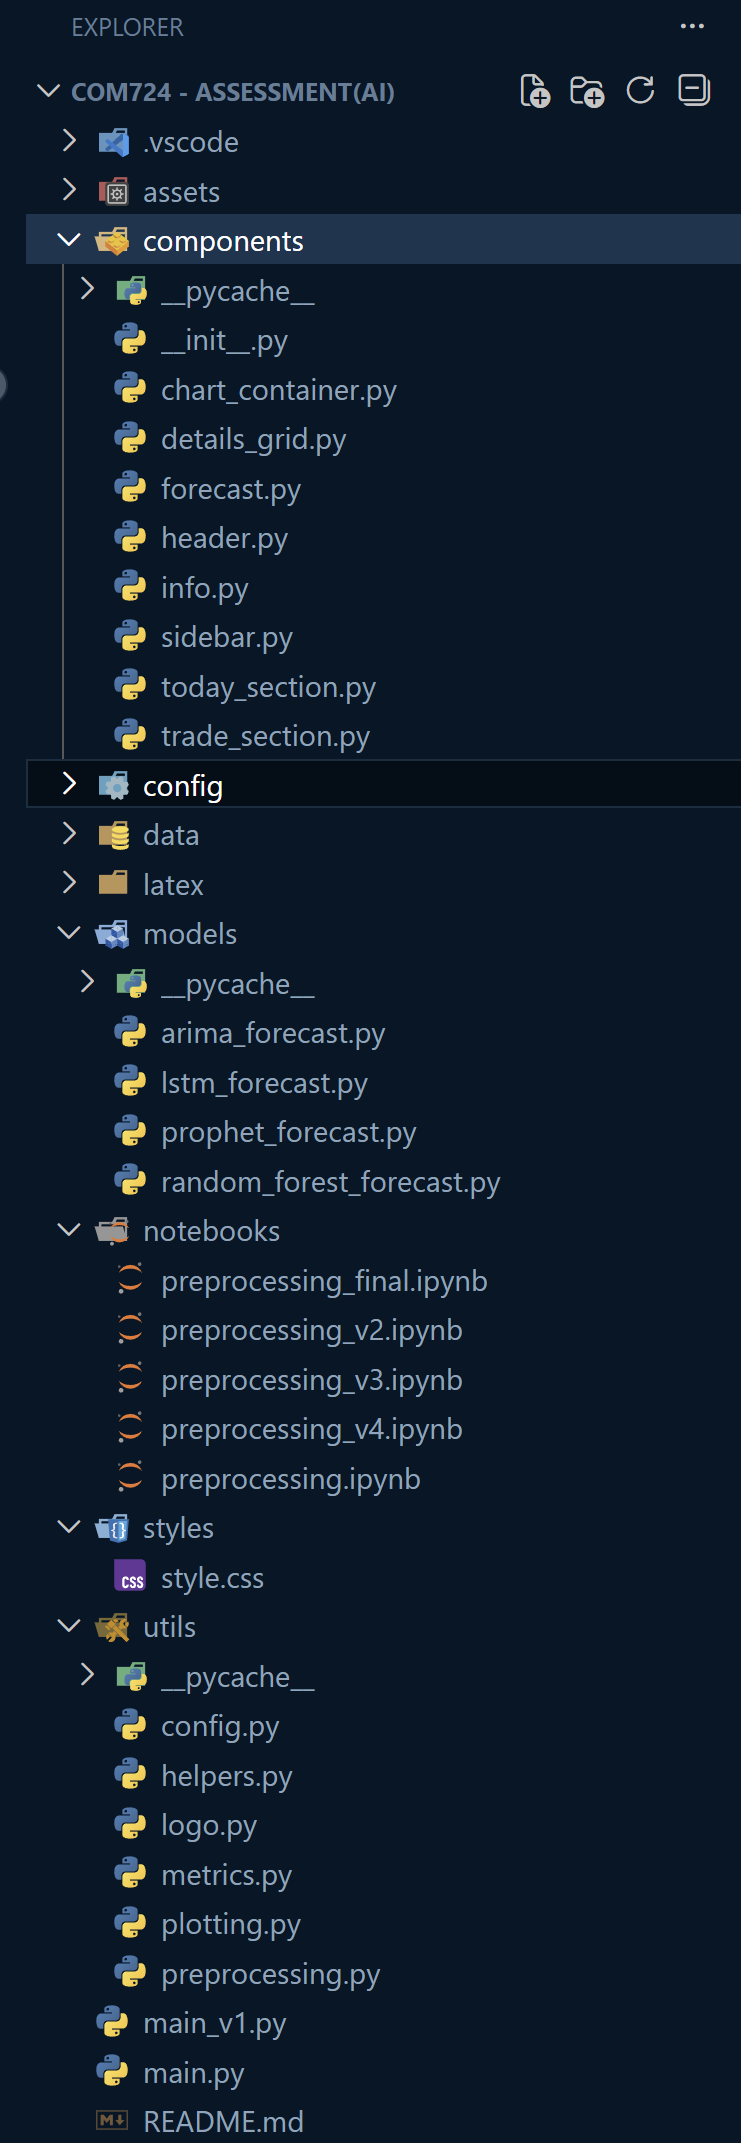
\includegraphics[width=0.35\textwidth]{../assets/system_architecture.png}
\caption{High-level system architecture showing modular components}
\label{fig:architecture}
\end{figure}

\section{Project Folder Structure}

The project directory is organised into logical folders, each responsible for a specific aspect of the system.

\subsection{\texttt{components/}}

This folder contains all user interface components used in the Streamlit application. It is responsible for structuring and displaying different sections of the dashboard, ensuring a clear separation between presentation and application logic.

\subsection{\texttt{models/}}

The \texttt{models} folder contains implementations of multiple forecasting algorithms. Each model is isolated within this directory, allowing easy comparison between different predictive approaches and supporting extensibility.

\subsection{\texttt{utils/}}

This directory provides shared utility functions used throughout the system. It supports data preprocessing, evaluation, configuration management, and plotting, helping to reduce code duplication and improve consistency.

\subsection{\texttt{data/}}

The \texttt{data} folder stores cryptocurrency datasets used for training, testing, and forecasting. It acts as the central location for all raw and processed data files.

\subsection{\texttt{notebooks/}}

This folder contains Jupyter notebooks used during exploratory data analysis and experimentation. It documents the iterative development of preprocessing techniques and feature engineering strategies.

\subsection{\texttt{styles/}}

The \texttt{styles} directory holds custom styling files that define the visual appearance of the Streamlit application, enhancing readability and user experience.

\subsection{\texttt{assets/}}

The \texttt{assets} folder stores static resources such as images, logos, and diagrams used in the application and project documentation.

\subsection{\texttt{latex/}}

This directory contains LaTeX source files used to produce the academic report associated with the project.

\chapter*{Data Collection and Preprocessing}
\addcontentsline{toc}{chapter}{Data Collection and Preprocessing}

Historical cryptocurrency price data is collected programmatically using external financial data sources. The dataset consists of daily open, high, low, close, and volume values, which are then passed through a preprocessing pipeline before being used for forecasting.

\section{Data Collection}

The following code snippet demonstrates how historical price data is downloaded, stored locally, and passed to the preprocessing function.

\begin{lstlisting}[caption={Cryptocurrency data collection and storage}]
import yfinance as yf

try:
    data = yf.download(ticker, START_DATE, TODAY)
    data.reset_index(inplace=True)

    if isinstance(data.columns, pd.MultiIndex):
        data.columns = [col[0] for col in data.columns]

    base_dir = "data"
    ticker_dir = os.path.join(base_dir, ticker)
    os.makedirs(ticker_dir, exist_ok=True)

    file_name = f"{ticker}_from_{START_DATE}_till_{TODAY}.csv"
    file_path = os.path.join(ticker_dir, file_name)

    data.to_csv(file_path, index=False)
    print(f"Data saved to: {file_path}")

    btc_preprocessed = preprocessing(data)
    return btc_preprocessed
\end{lstlisting}

\section{Preprocessing}

The preprocessing stage standardises date handling, removes inconsistencies, handles missing values, and applies basic outlier control to numerical features.

\begin{lstlisting}[caption={Data preprocessing function}]
def preprocessing(data: pd.DataFrame) -> pd.DataFrame:
    df = data.copy()

    if 'Date' in df.columns:
        df['Date'] = pd.to_datetime(df['Date'])
        df.set_index('Date', inplace=True)

    df.ffill(inplace=True)
    df.drop_duplicates(inplace=True)

    numeric_cols = df.select_dtypes(include=[np.number]).columns.tolist()

    for col in numeric_cols:
        lower = df[col].quantile(0.05)
        upper = df[col].quantile(0.95)
        df[col] = df[col].clip(lower, upper)

    return df
\end{lstlisting}

% ======================
% FEATURE ENGINEERING
% ======================

\chapter*{Exploratory Data Analysis}

\addcontentsline{toc}{chapter}{Exploratory Data Analysis}

Exploratory Data Analysis (EDA) was conducted to understand the characteristics, distributions, and relationships within the cryptocurrency price data before applying forecasting models. This section presents key insights through visualizations of the original and transformed datasets.

\section{Feature Correlation Analysis}

\begin{figure}[H]
\centering
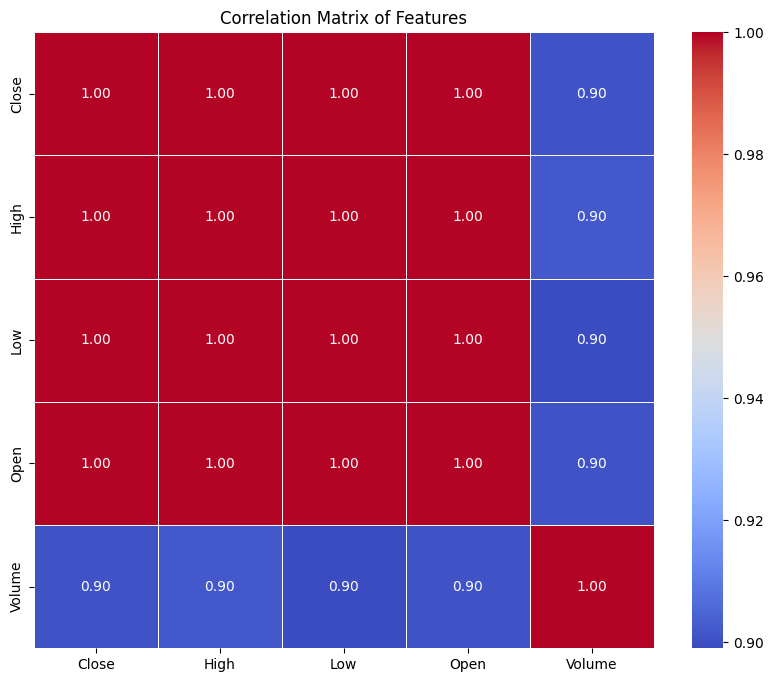
\includegraphics[width=0.8\textwidth]{../assets/correlation_matrix.png}
\caption{Correlation Matrix of Cryptocurrency Price Features}
\label{fig:correlation_matrix}
\end{figure}

Figure \ref{fig:correlation_matrix} presents a correlation heatmap of the primary price features: Close, High, Low, Open, and Volume. The visualization reveals near-perfect positive correlation ($\approx$1.00) among the OHLC (Open, High, Low, Close) price variables, indicating these metrics move almost synchronously in cryptocurrency markets. Volume demonstrates a strong positive correlation of 0.90 with price metrics, suggesting trading activity is closely tied to price movements. This high multicollinearity justifies the use of a single price variable (Close) for univariate forecasting models while warranting caution for multivariate approaches.

\section{Data Transformation Analysis}

\begin{figure}[H]
\centering
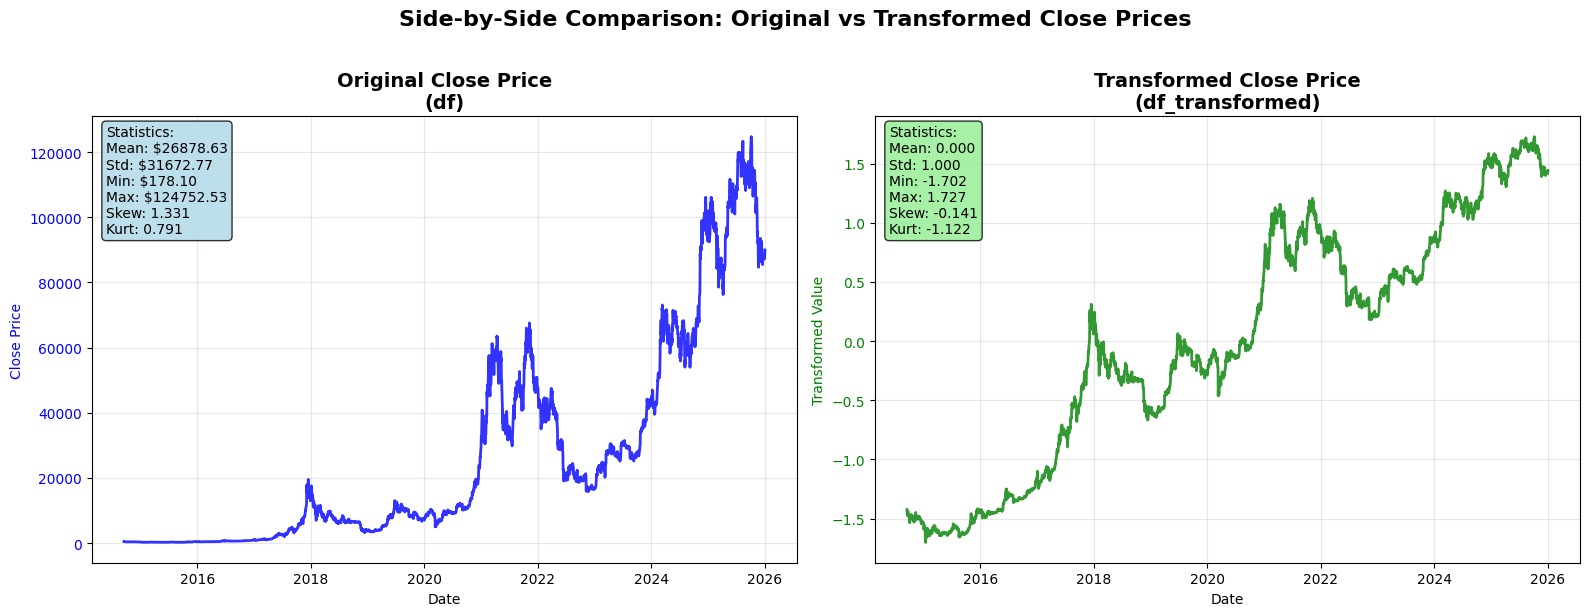
\includegraphics[width=1.0\textwidth]{../assets/distribution_comparison.png}
\caption{Comparison of Original vs Transformed Close Price Distributions}
\label{fig:distribution_comparison}
\end{figure}

Figure \ref{fig:distribution_comparison} illustrates the effect of the Yeo-Johnson transformation applied to normalize the price distribution. The original Close price exhibits significant positive skewness (1.331) and kurtosis (0.791), with a wide range from \$178.10 to \$124,752.53. After transformation, the data achieves near-zero mean and unit standard deviation, with skewness reduced to -0.141 and kurtosis to -1.122. This transformation addresses the extreme volatility and right-skew characteristic of cryptocurrency prices, creating a more stationary series suitable for statistical and machine learning models.

\section{Distribution Visualization}

\begin{figure}[H]
\centering
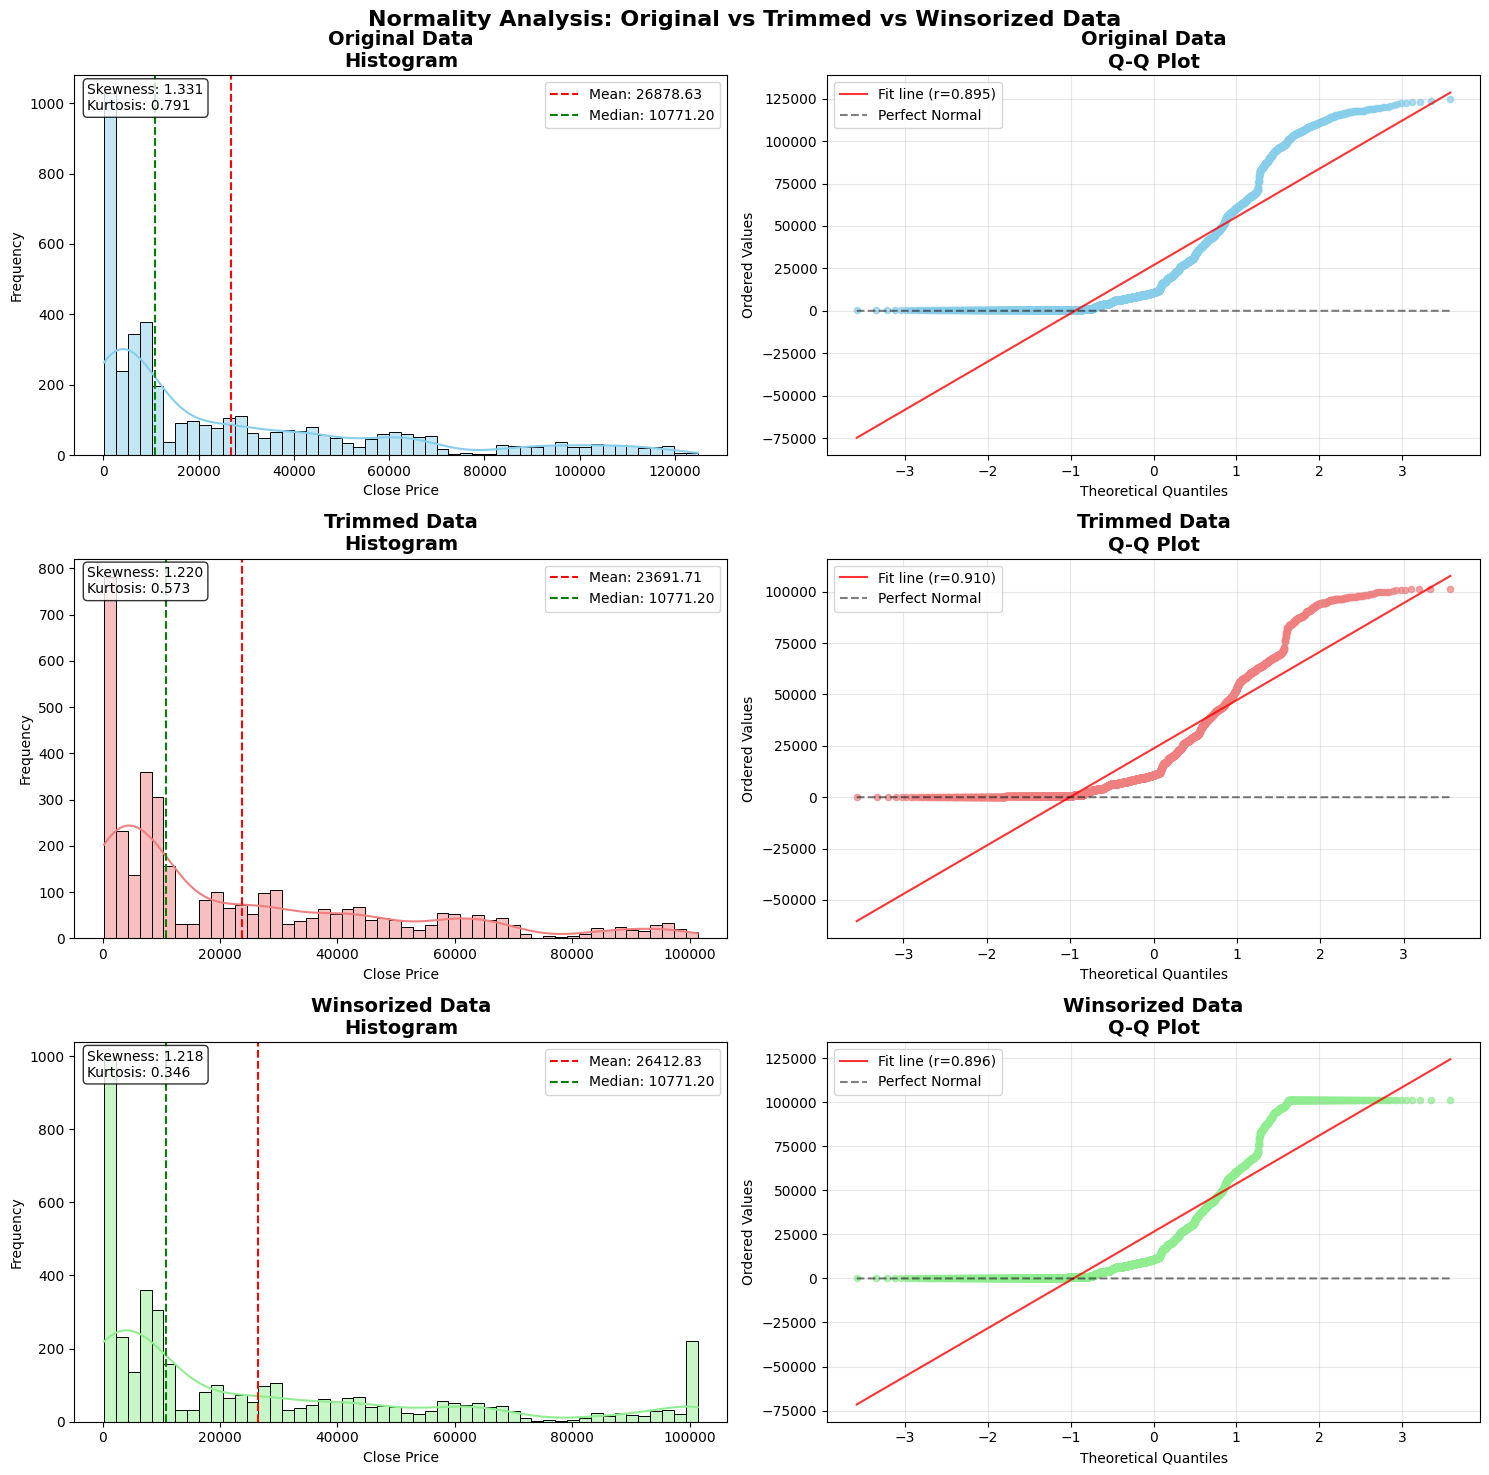
\includegraphics[width=1.0\textwidth]{../assets/distribution_visualization.png}
\caption{Comprehensive Distribution Analysis of Original and Transformed Prices}
\label{fig:distribution_visualization}
\end{figure}

Figure \ref{fig:distribution_visualization} provides a comprehensive view of price distributions through multiple visualization techniques. The top row presents the original Bitcoin price data: the histogram shows the heavily right-skewed distribution, the Q-Q plot reveals significant deviation from normality (especially in the upper tail), and the boxplot highlights numerous extreme outliers. The bottom row shows the transformed data: the histogram approaches a normal distribution, the Q-Q plot demonstrates much closer alignment with theoretical quantiles, and the boxplot shows reduced outlier presence. These visualizations confirm that the transformation successfully addresses the non-normality and heteroscedasticity inherent in cryptocurrency price data, creating a more suitable input for forecasting algorithms.

The EDA findings guided several critical modeling decisions: (1) the use of univariate approaches given high feature correlation, (2) the application of appropriate transformations to achieve stationarity, and (3) the selection of models robust to residual non-linearity and volatility. These insights formed the foundation for the feature engineering and model selection processes described in subsequent chapters.

\chapter*{Forecasting Models}
\addcontentsline{toc}{chapter}{Forecasting Models}

\section{ARIMA}
\subsection{Conceptual Overview}
The AutoRegressive Integrated Moving Average (ARIMA) model is a classical statistical approach that captures linear temporal dependencies through autoregressive (AR), differencing (I), and moving average (MA) components. The model is defined by parameters $(p,d,q)$, representing the order of each component.

\subsection{Suitability for Cryptocurrency Data}
ARIMA serves as a foundational benchmark due to its simplicity and interpretability. Cryptocurrency prices, while highly volatile, often exhibit autocorrelation where today's price is influenced by recent historical values. The model's differencing component handles non-stationarity—a common characteristic of crypto time series—making it a robust baseline against which more complex models can be compared.

\subsection{Feature Engineering Approach}
ARIMA requires no explicit feature engineering. The model is fitted directly on the univariate \texttt{Close} price series. Stationarity is ensured through differencing ($d$), while temporal patterns are captured via lagged terms ($p$) and error smoothing ($q$). The implementation uses \texttt{auto\_arima} to automatically determine optimal $(p,d,q)$ parameters, eliminating manual configuration.

\subsection{Evaluation Framework}

\begin{figure}[H]
\centering
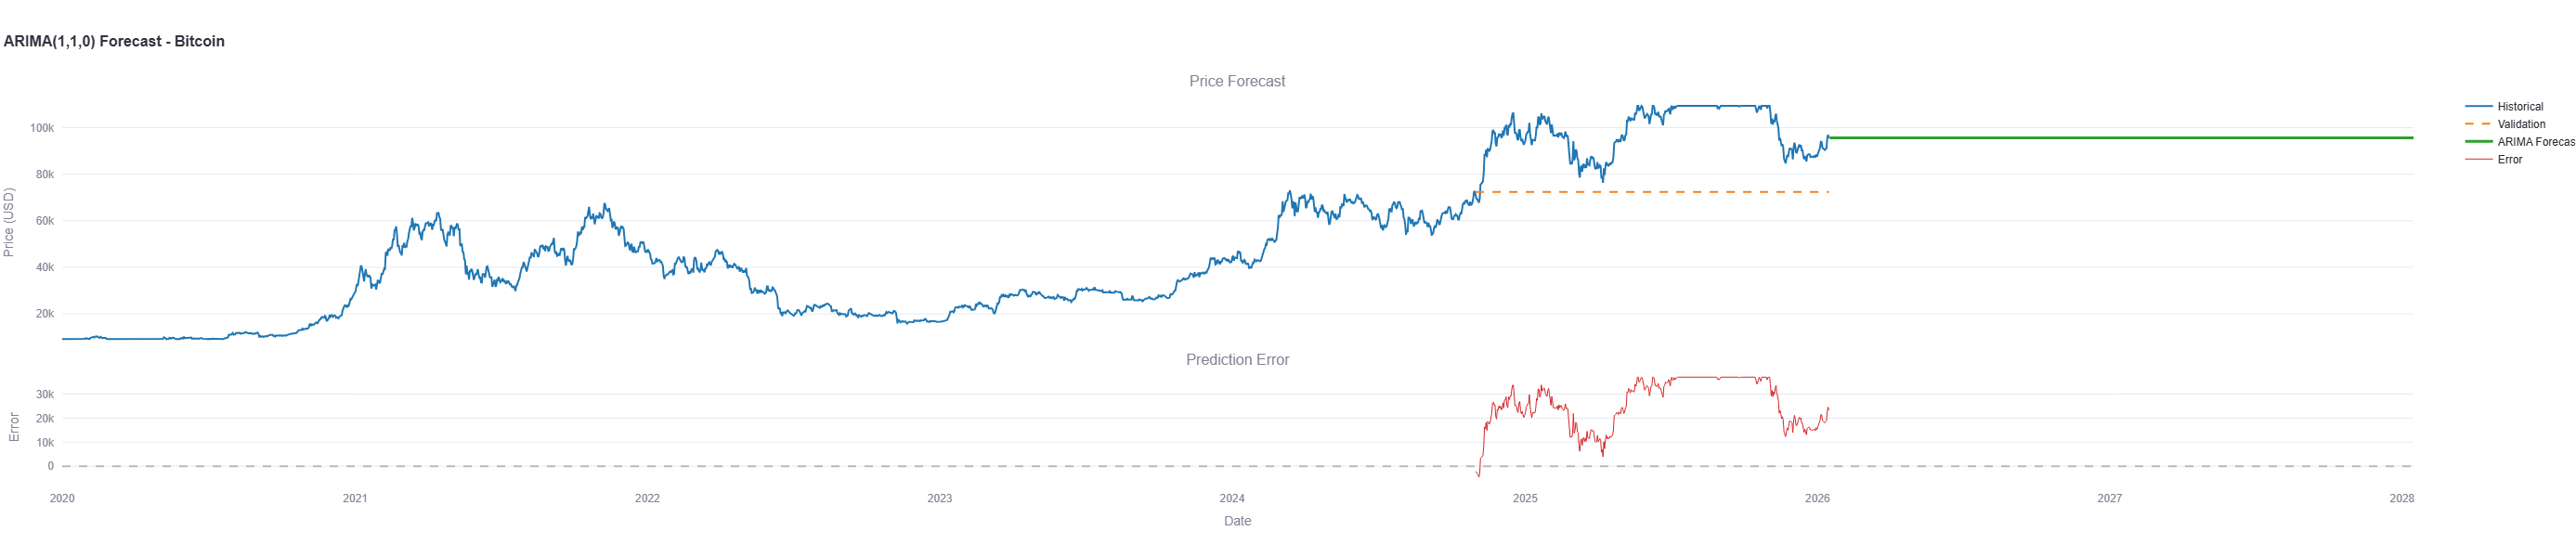
\includegraphics[width=1.0\textwidth]{../assets/arima.png}
\caption{Forecasting architecture of ARIMA model}
\label{fig:arima}
\end{figure}

Model performance is assessed using RMSE, MAE, R\textsuperscript{2} Score, and MAPE. These metrics quantify prediction accuracy, error magnitude, explanatory power, and percentage deviation respectively, providing a multi-dimensional view of forecast quality on a held-out test set (20\% of data).

\begin{table}[h]
\centering
\caption{Evaluation Metrics for Bitcoin using ARIMA (1,1,0) Model}
\label{tab:arima-bitcoin-metrics}
\begin{tabular}{lr}
\toprule
\textbf{Metric} & \textbf{Value} \\
\midrule
RMSE & 28010.47 \\
MAE & 26261.12 \\
R\textsuperscript{2} & -6.8848 \\
MAPE & 25.87\% \\
\bottomrule
\end{tabular}
\end{table}

\section{Prophet}
\subsection{Conceptual Overview}
Prophet is an additive regression model developed by Facebook for forecasting time series with strong seasonal patterns. It decomposes the series into trend, seasonality, and holiday components using a Bayesian curve-fitting approach.

\subsection{Suitability for Cryptocurrency Data}
Prophet excels at capturing recurring patterns and adapting to structural breaks—both relevant to cryptocurrency markets which exhibit intra-week and intra-year seasonalities (e.g., weekend effects, quarterly trends). Its ability to handle missing data and outliers makes it resilient to the noisy, irregular observations common in crypto datasets.

\subsection{Feature Engineering Approach}
Prophet requires minimal preprocessing: only a date column (\texttt{ds}) and a target column (\texttt{y}). The model internally constructs Fourier series for seasonal terms and changepoints for trend shifts. Yearly and weekly seasonality are enabled, while daily seasonality is disabled given the daily frequency of the data.

\subsection{Evaluation Framework}

\begin{figure}[H]
\centering
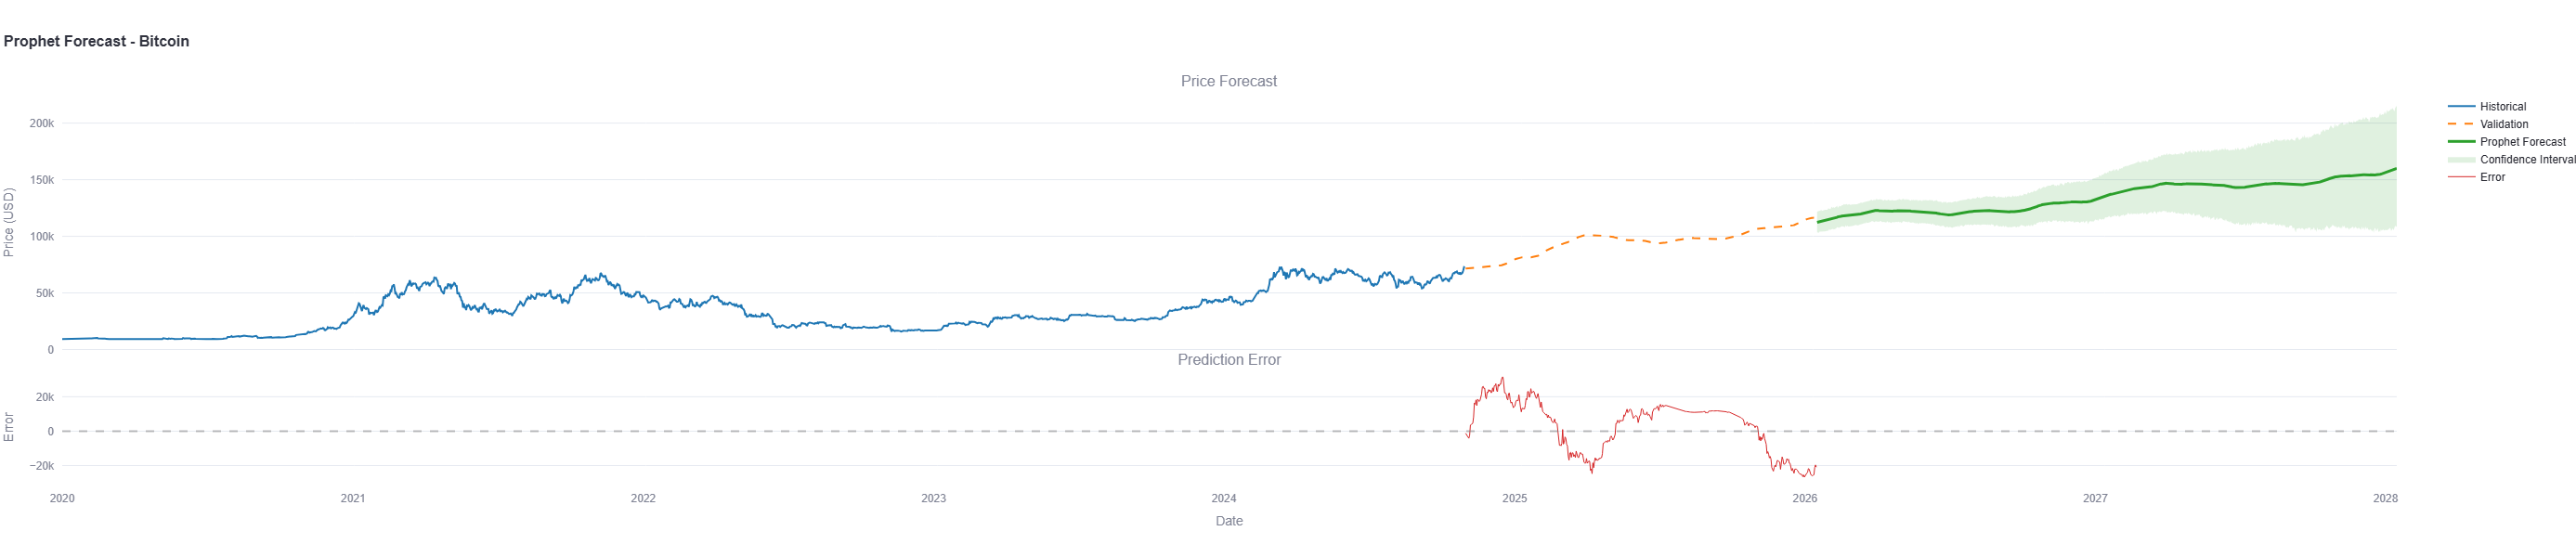
\includegraphics[width=1.0\textwidth]{../assets/prophet.png}
\caption{Forecasting architecture of Prophet model}
\label{fig:prophet}
\end{figure}

Performance is measured using the same quartet of metrics (RMSE, MAE, R\textsuperscript{2}, MAPE) applied to a time-based validation split. Prophet also outputs prediction intervals, though these are used for visualization rather than formal evaluation in this implementation.

\begin{table}[h]
\centering
\caption{Evaluation Metrics for Bitcoin using Prophet Model}
\label{tab:prophet-bitcoin-metrics}
\begin{tabular}{lr}
\toprule
\textbf{Metric} & \textbf{Value} \\
\midrule
RMSE &  15106.45\\
MAE &  13565.15\\
R\textsuperscript{2} &  -1.2934\\
MAPE &  3.14\%\\
\bottomrule
\end{tabular}
\end{table}

\section{LSTM}
\subsection{Conceptual Overview}
Long Short-Term Memory (LSTM) networks are a type of recurrent neural network (RNN) designed to capture long-range temporal dependencies through gated memory cells. Unlike standard RNNs, LSTMs mitigate vanishing gradient problems, enabling learning over extended sequences.

\subsection{Suitability for Cryptocurrency Data}
Cryptocurrency markets exhibit complex, nonlinear dependencies that traditional statistical models may miss. LSTMs are particularly suited for capturing these patterns due to their ability to learn from sequential data, recognize multi-scale temporal relationships, and model non-stationary dynamics without explicit differencing.

\subsection{Feature Engineering Approach}
The \texttt{Close} price is MinMax-scaled and restructured into overlapping sequences of 60 time steps, with each sequence predicting the next day's price. The 3D input format \texttt{[samples, timesteps, features]} allows the LSTM to learn from the temporal ordering inherently, requiring no handcrafted lag or statistical features.

\subsection{Evaluation Framework}

\begin{figure}[H]
\centering
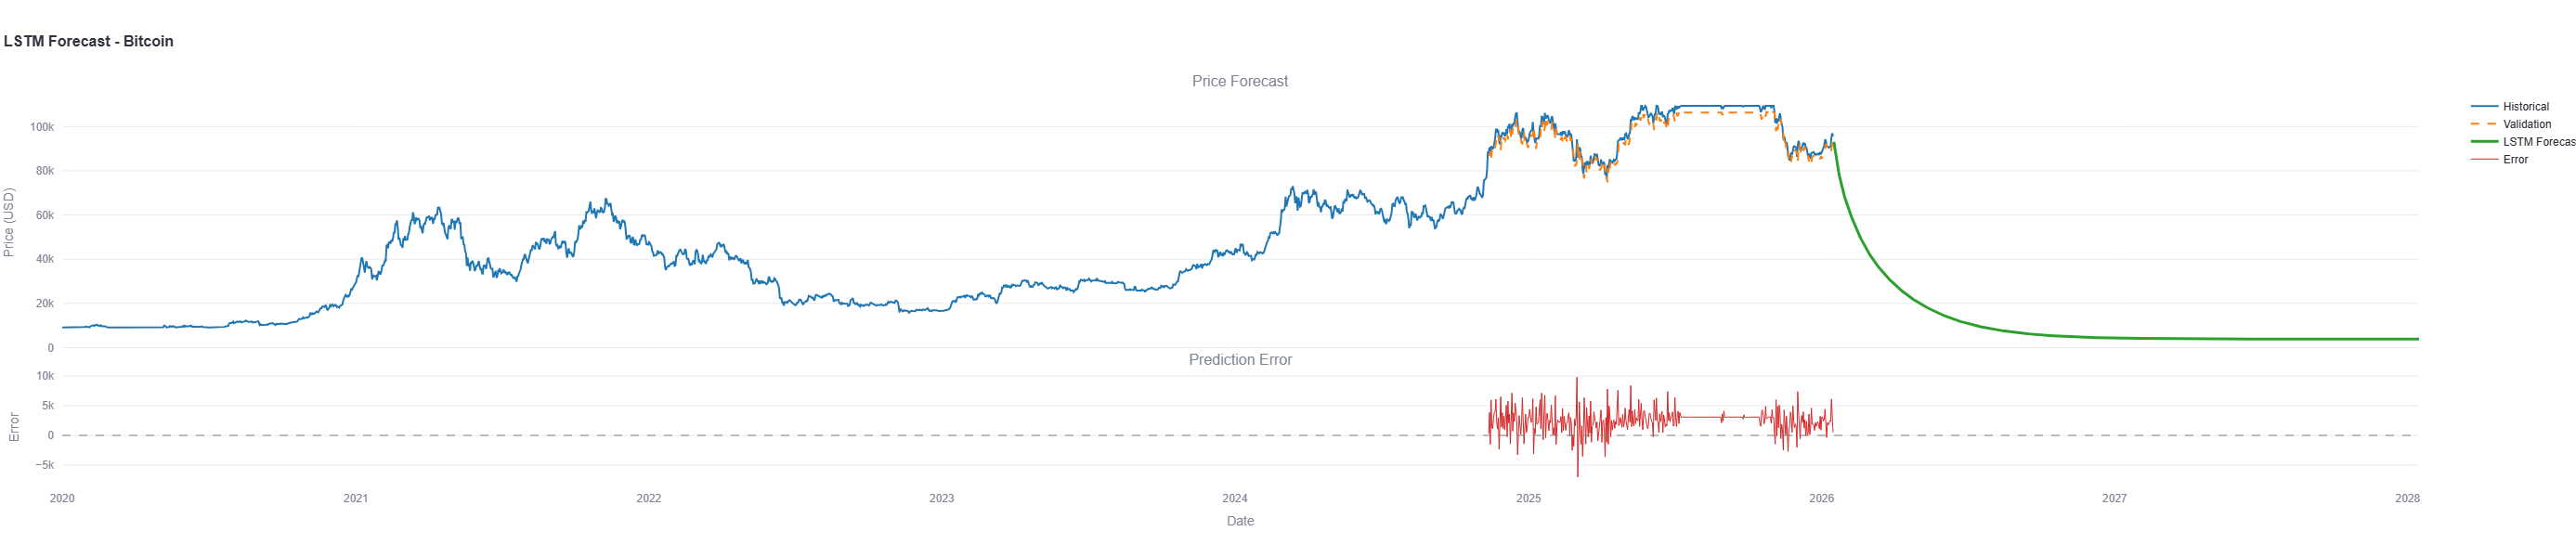
\includegraphics[width=1.0\textwidth]{../assets/lstm.png}
\caption{Forecasting architecture of LSTM model}
\label{fig:lstm}
\end{figure}

Model validation follows a time-series split, with 20\% of sequences held out for testing. Performance metrics (RMSE, MAE, R\textsuperscript{2}, MAPE) are computed after inverse-transforming predictions to the original price scale, ensuring interpretability.

\begin{table}[h]
\centering
\caption{Evaluation Metrics for Bitcoin using LSTM Model}
\label{tab:lstm-bitcoin-metrics}
\begin{tabular}{lr}
\toprule
\textbf{Metric} & \textbf{Value} \\
\midrule
RMSE &  3161.26\\
MAE &  2772.81\\
R\textsuperscript{2} &  0.8812\\
MAPE &  2.78\%\\
\bottomrule
\end{tabular}
\end{table}

\section{Random Forest}
\subsection{Conceptual Overview}
Random Forest is an ensemble machine learning method that constructs multiple decision trees during training and outputs the mean prediction of individual trees. It handles nonlinear relationships and provides feature importance estimates, making it robust to overfitting.

\subsection{Suitability for Cryptocurrency Data}
The model's ability to learn complex interactions between multiple input features makes it effective for cryptocurrency forecasting, where price movements result from intertwined technical, temporal, and volatility factors. Its resistance to outliers and noise aligns well with crypto market conditions.

\subsection{Feature Engineering Approach}
Explicit feature engineering is essential. This includes lagged prices (1–30 days), rolling statistics (moving averages, standard deviations over 7–60 days), and derived ratios (e.g., price-to-moving-average). These features encode trend, volatility, momentum, and mean-reversion signals, transforming the univariate series into a multidimensional representation suitable for tree-based learning.

\subsection{Evaluation Framework}

\begin{figure}[H]
\centering
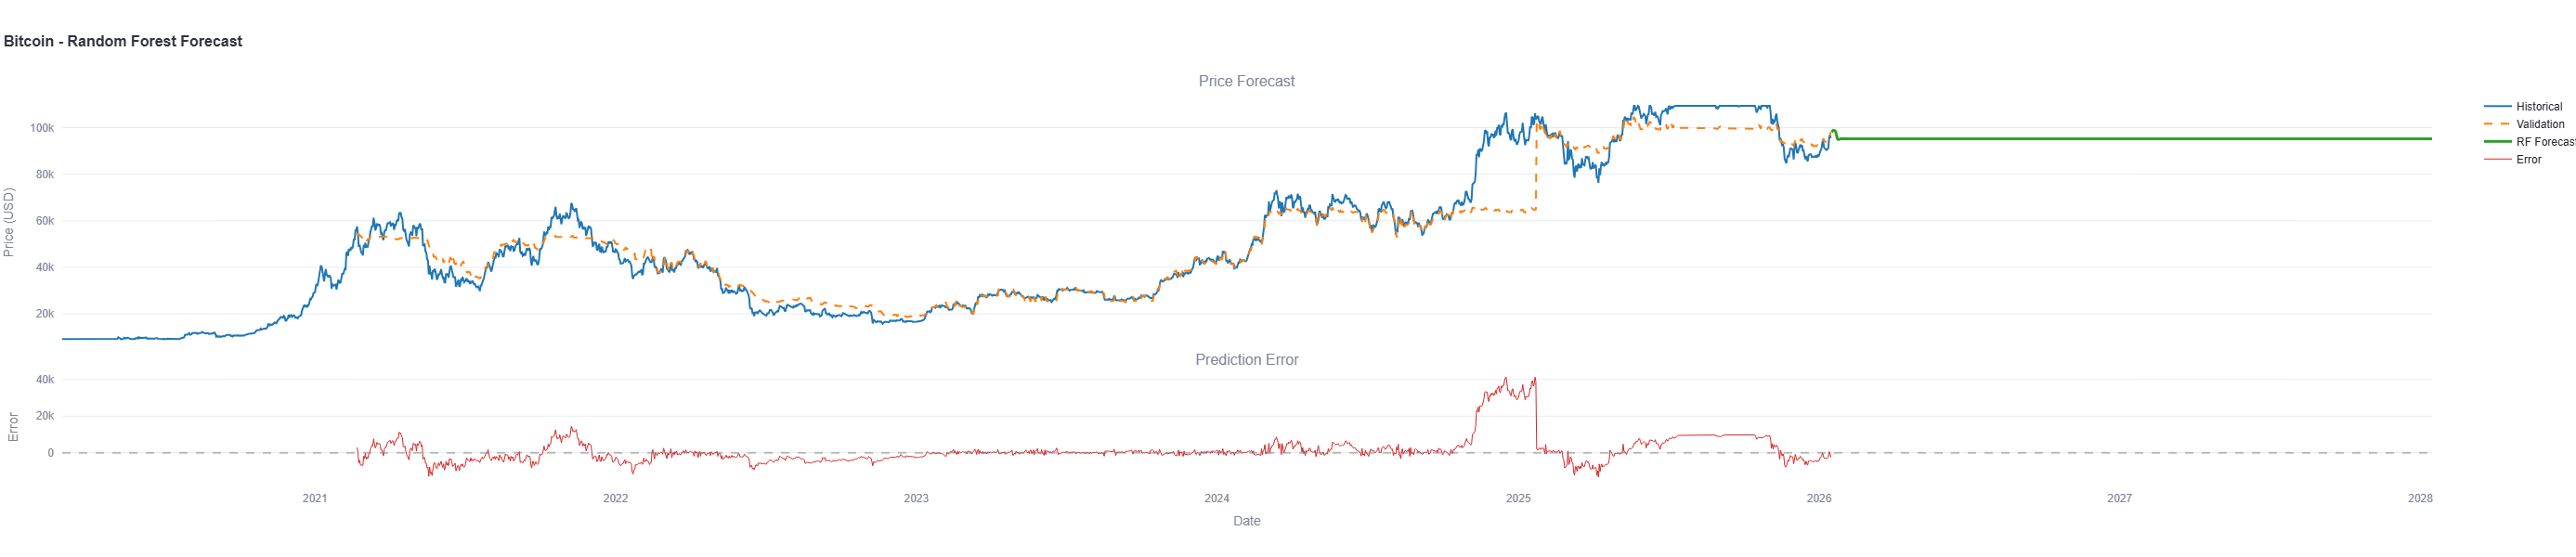
\includegraphics[width=1.0\textwidth]{../assets/randomforest.png}
\caption{Forecasting architecture of Random Forest model}
\label{fig:randomforest}
\end{figure}

A time-series cross-validation with 5 splits is employed to respect temporal ordering. Standard regression metrics (RMSE, MAE, R\textsuperscript{2}, MAPE) are computed across all validation folds, providing a robust estimate of out-of-sample performance.

\begin{table}[h]
\centering
\caption{Evaluation Metrics for Bitcoin using Random Forest Model}
\label{tab:rf-bitcoin-metrics}
\begin{tabular}{lr}
\toprule
\textbf{Metric} & \textbf{Value} \\
\midrule
RMSE &  7976.75\\
MAE &  4544.81\\
R\textsuperscript{2} &  0.9248\\
MAPE &  8.26\%\\
\bottomrule
\end{tabular}
\end{table}

\chapter*{Streamlit Application}
\addcontentsline{toc}{chapter}{Streamlit Application}

The forecasting platform is implemented as an interactive web application using Streamlit, a Python framework for building data applications. The interface is organized into four main sections that guide users through the forecasting workflow, from configuration to results visualization.

\section{Sidebar Navigation and Configuration}

\begin{figure}[H]
\centering
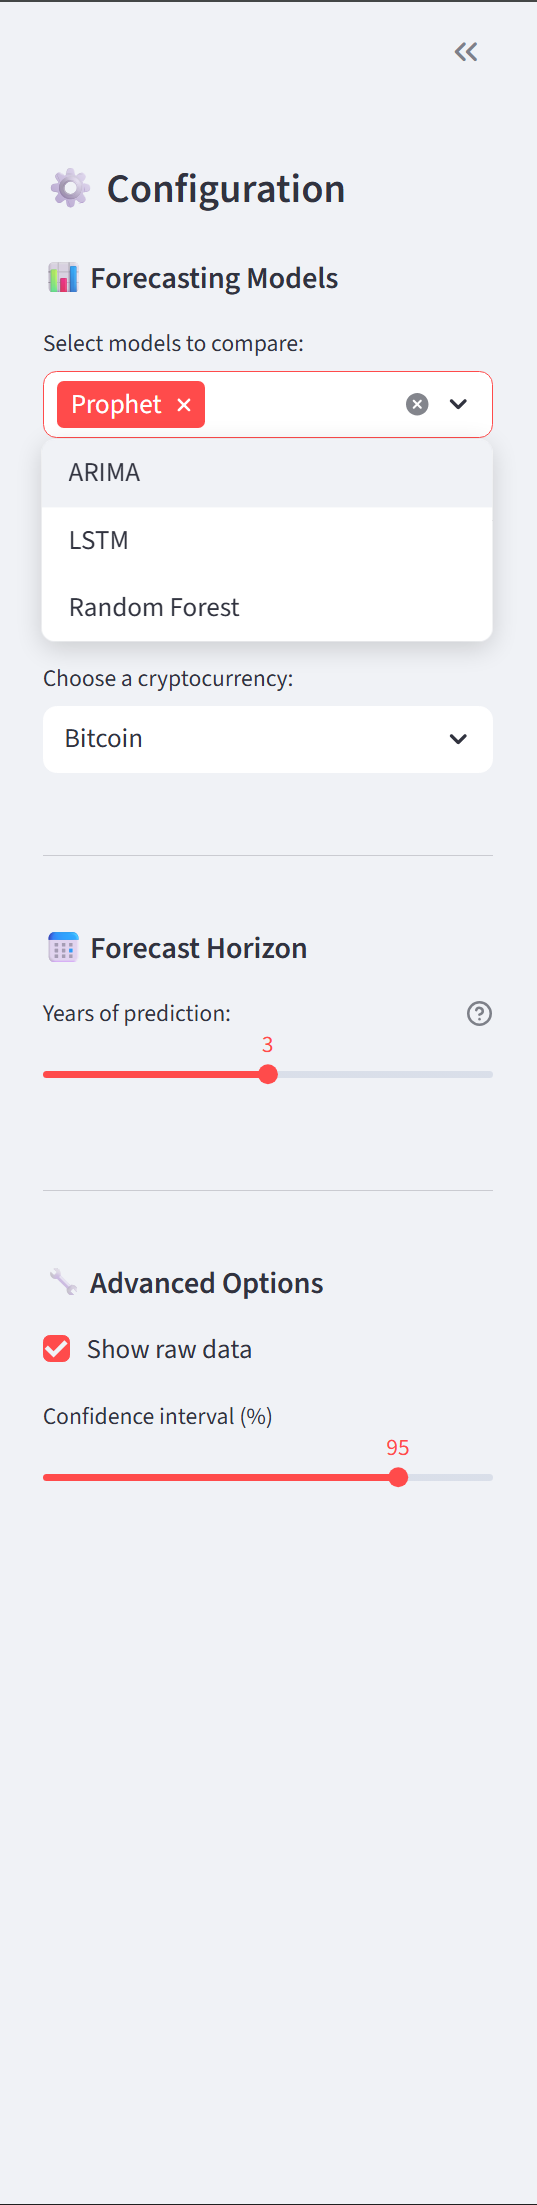
\includegraphics[width=0.3\textwidth]{../assets/sidenav.png}
\caption{Sidebar Configuration Panel for Model and Forecast Settings}
\label{fig:sidebar_config}
\end{figure}

The left sidebar (Figure \ref{fig:sidebar_config}) serves as the central control panel for the forecasting system. Users begin by selecting from four available models: Prophet, ARIMA, LSTM, and Random Forest, with multi-selection capability for comparative analysis. The cryptocurrency selection dropdown includes major assets such as Bitcoin, Ethereum, Solana, and Ripple. Forecast horizons are configured in years (1-5), with advanced options including confidence interval settings (80-95\%) and raw data display toggles. This modular design allows users to customize the forecasting scenario according to their analytical needs before any computation begins.

\section{Header and Market Information Display}

\begin{figure}[H]
\centering
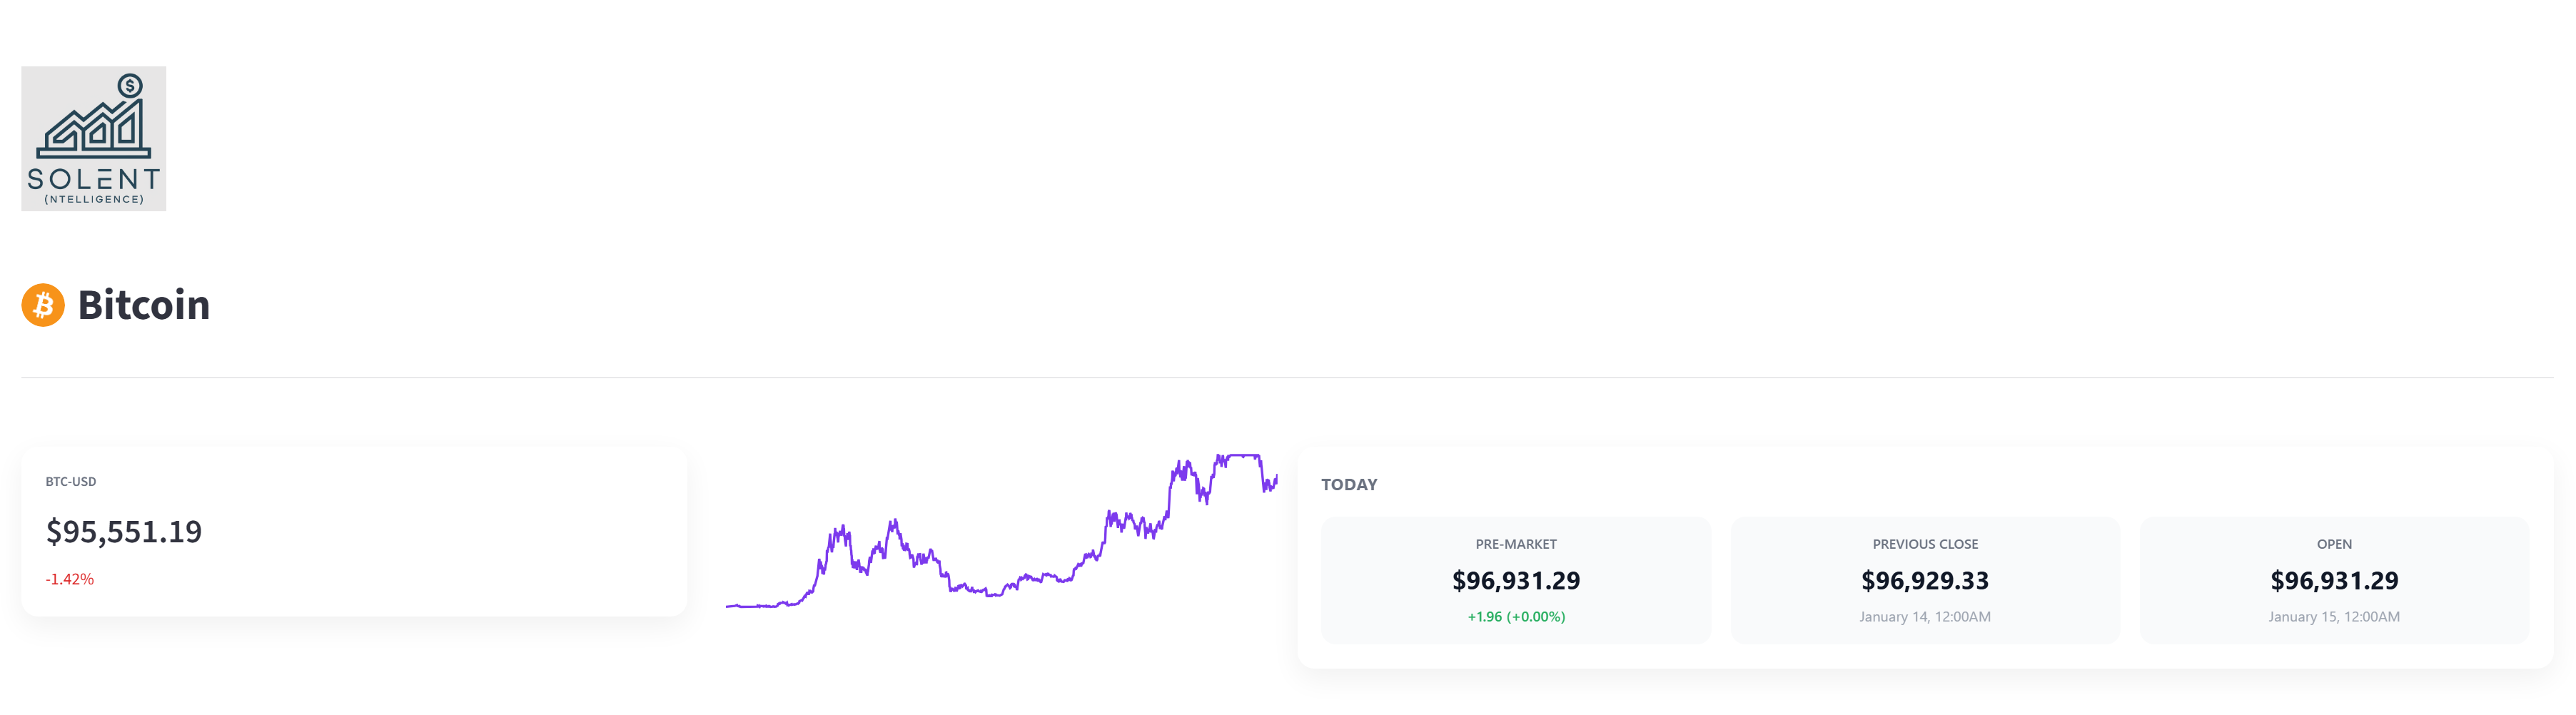
\includegraphics[width=1.0\textwidth]{../assets/header.png}
\caption{Market Overview Header with Real-time Cryptocurrency Metrics}
\label{fig:header_info}
\end{figure}

The header section (Figure \ref{fig:header_info}) provides immediate market context upon cryptocurrency selection. It displays the trading pair symbol (e.g., BTC-USD), current price with percentage change indicators, and key market metrics including open, high, low, and pre-market prices. This real-time information establishes the baseline against which forecasts are evaluated, helping users understand current market conditions before interpreting predictive outputs. The visual design employs color-coded changes (green/red) for quick sentiment assessment.

\section{Interactive Historical Chart Visualization}

\begin{figure}[H]
\centering
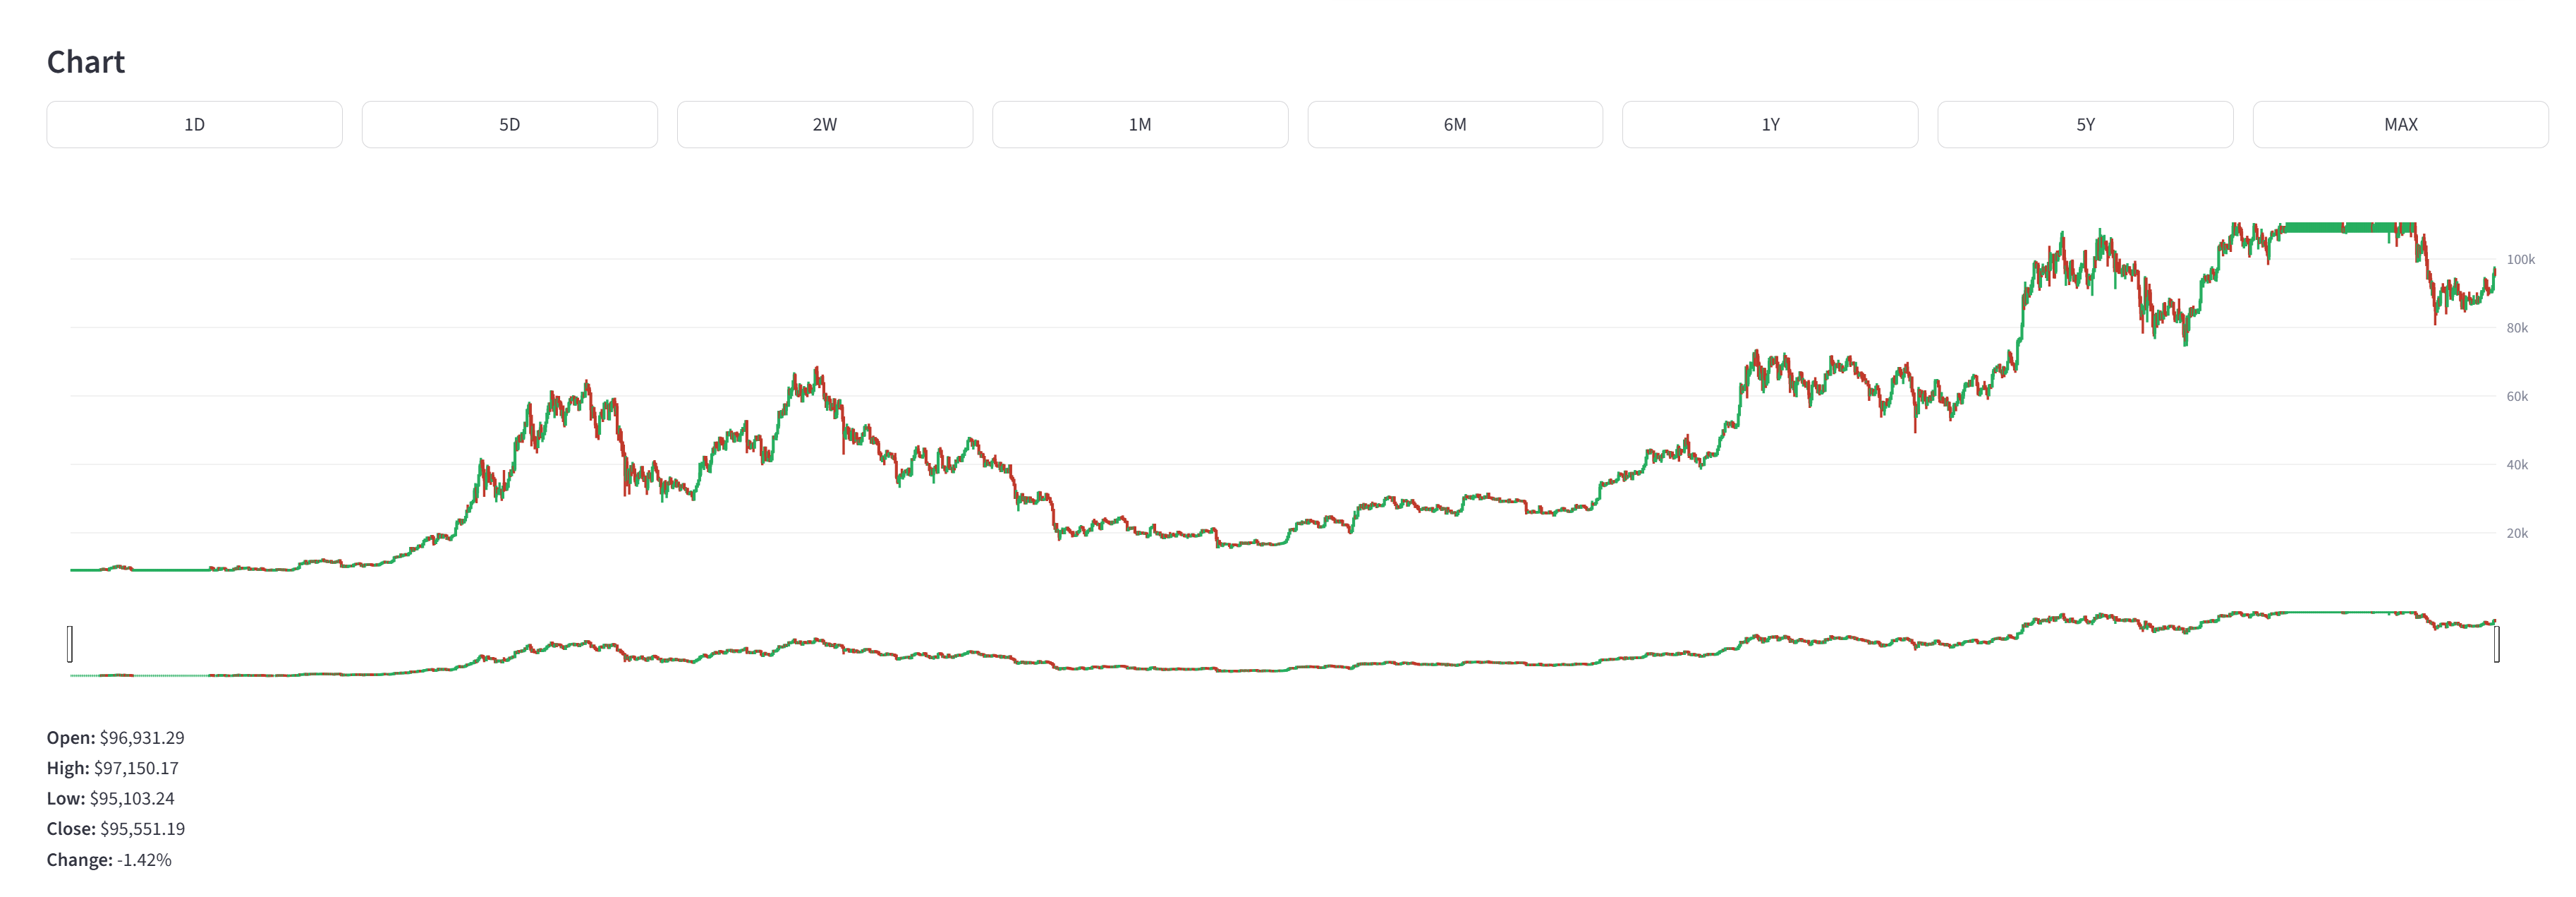
\includegraphics[width=1.0\textwidth]{../assets/chart.png}
\caption{Interactive Price Chart with Time Window Controls}
\label{fig:chart_section}
\end{figure}

The central chart section (Figure \ref{fig:chart_section}) offers interactive exploration of historical price data through a Plotly visualization. Users can adjust the time window using preset intervals (1D to MAX) or manually zoom and pan across the timeline. The chart displays OHLC (Open-High-Low-Close) data with hover tooltips showing detailed price information at specific points. This interactive component serves dual purposes: establishing historical context for the forecasts and allowing users to identify patterns, trends, and volatility regimes that may inform their interpretation of model predictions.

\section{Forecast Results and Model Comparison}

\begin{figure}[H]
\centering
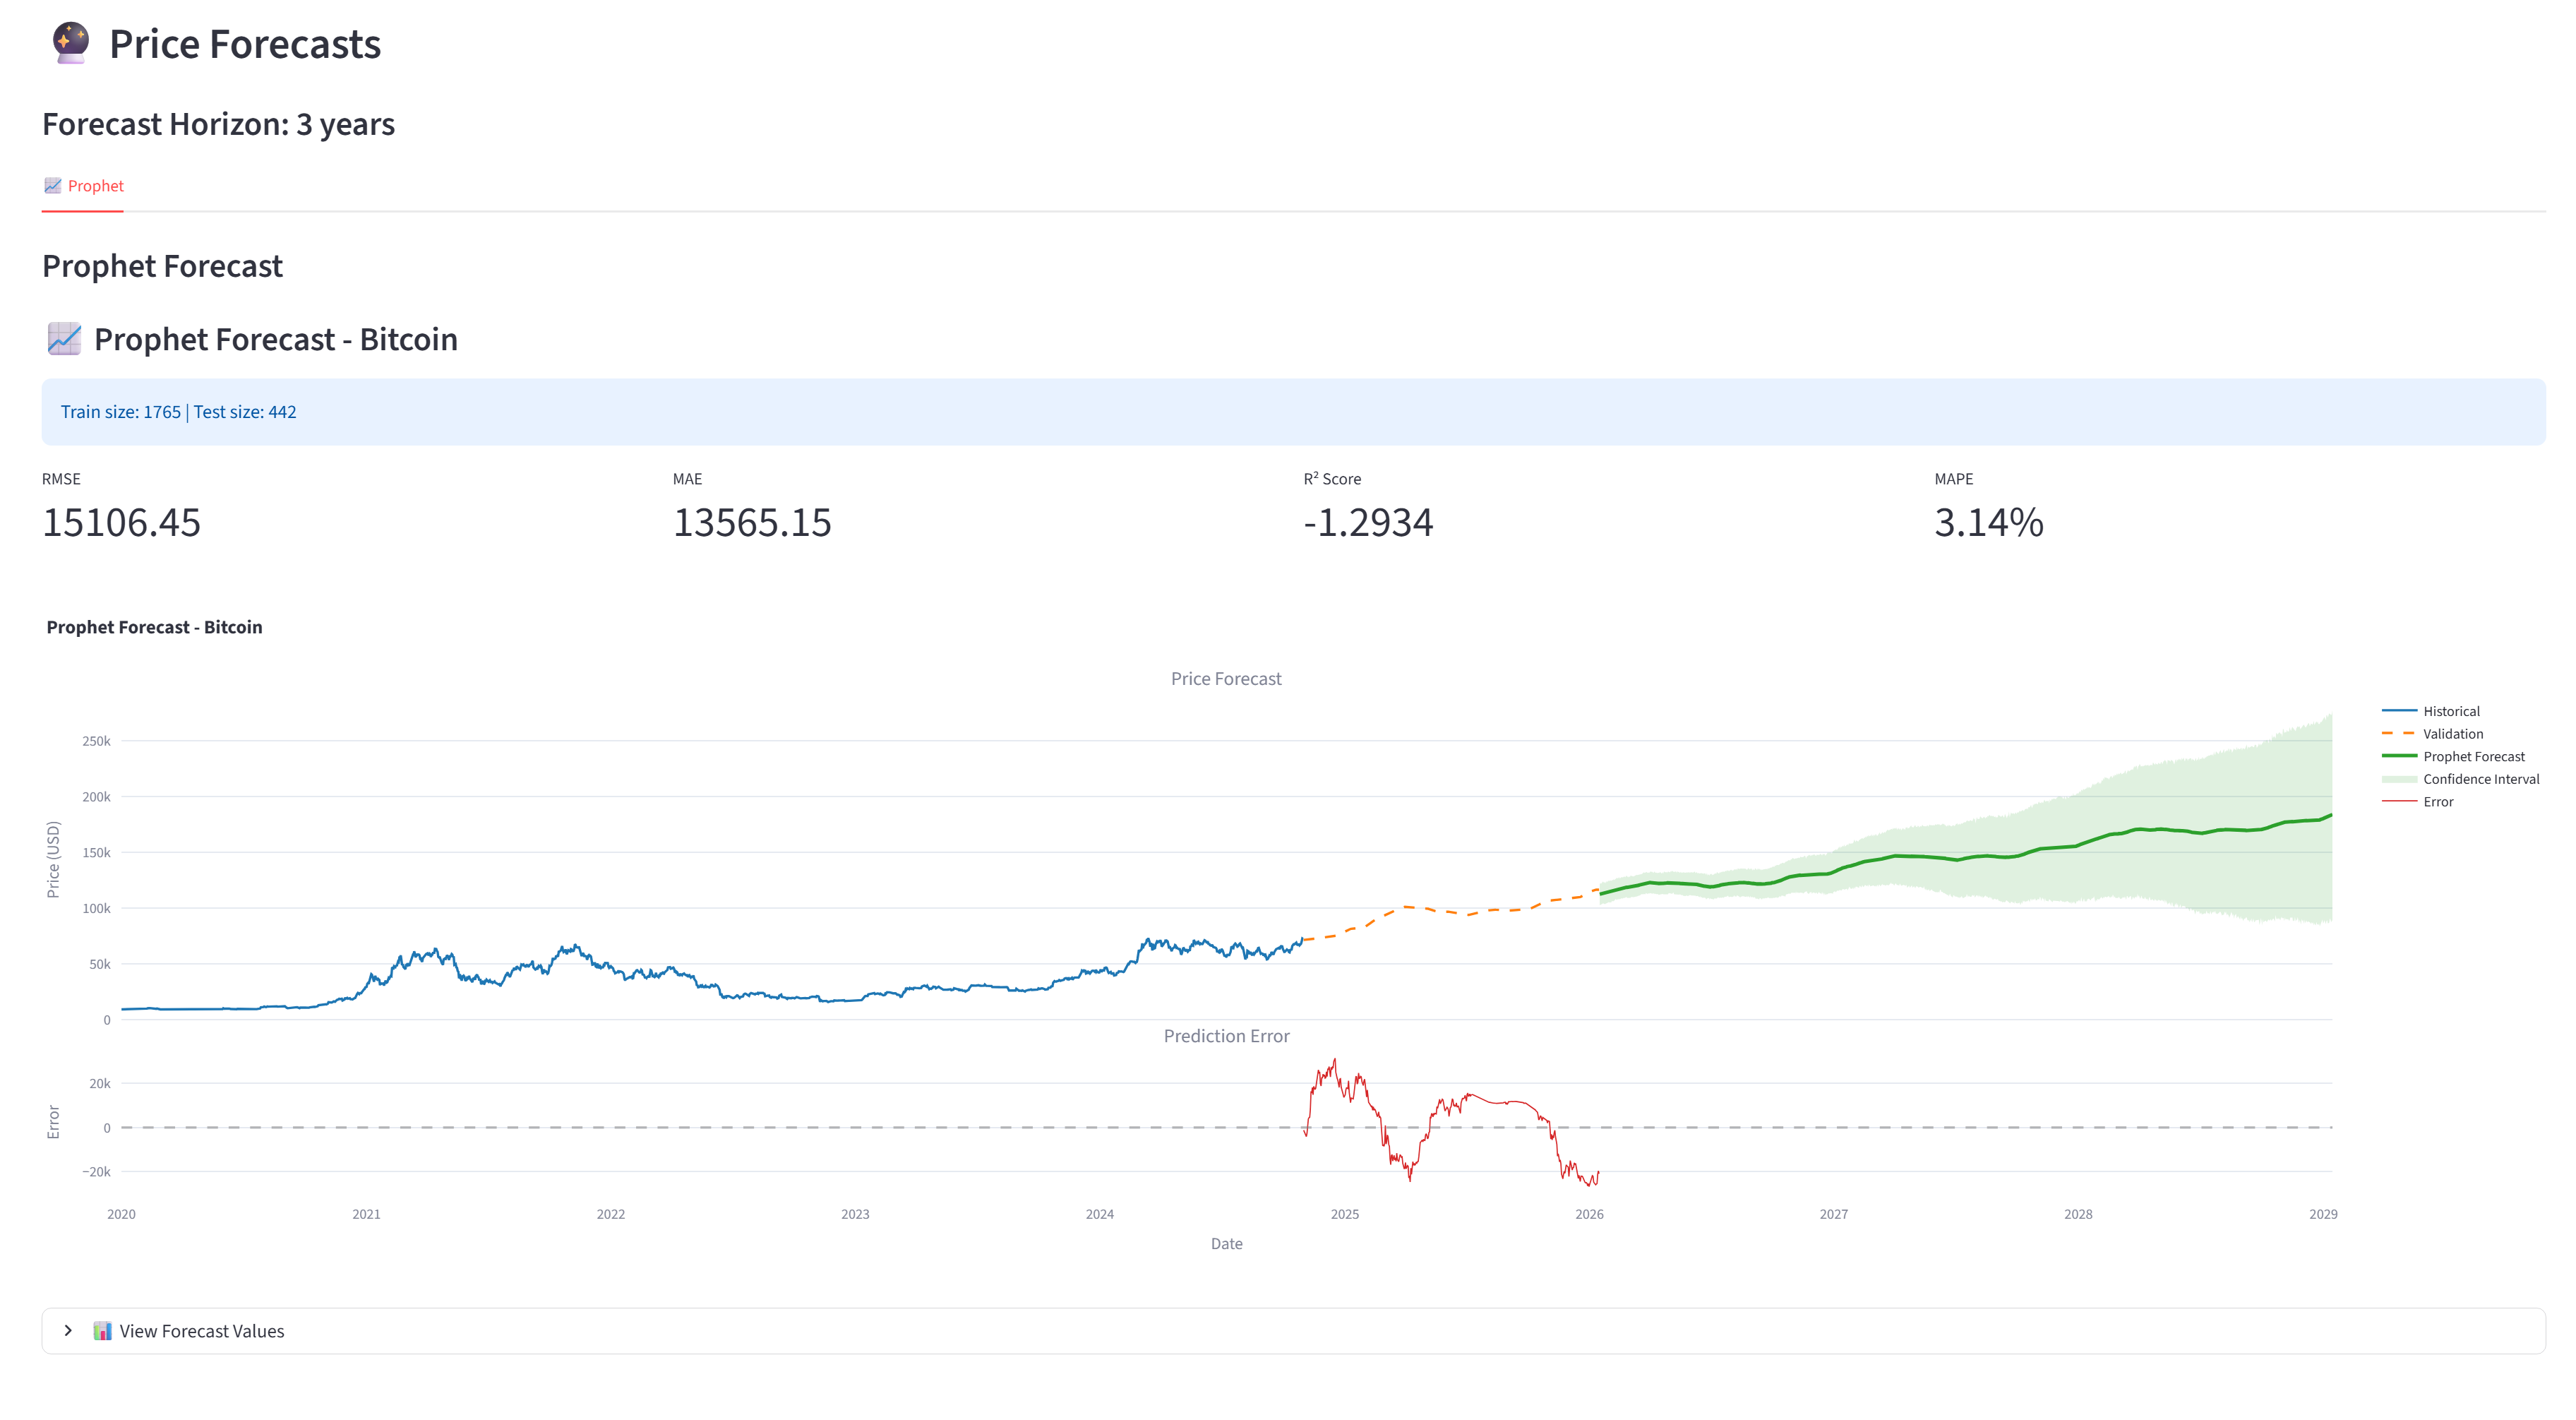
\includegraphics[width=1.0\textwidth]{../assets/forecast.png}
\caption{Forecast Visualization with Model Metrics and Predictions}
\label{fig:forecast_section}
\end{figure}

The forecast results section (Figure \ref{fig:forecast_section}) presents the analytical core of the application. Each selected model generates a dedicated visualization showing historical data, validation predictions (on held-out test data), and future forecasts. The two-panel layout includes: (1) a price forecast chart with confidence intervals, and (2) a prediction error plot showing model residuals. Below each visualization, a four-metric dashboard displays RMSE, MAE, R² Score, and MAPE, providing quantitative assessment of model performance. When multiple models are selected, these visualizations are stacked vertically, enabling direct comparison of forecasting approaches.

The application architecture follows a clear user journey: configuration -> market context -> historical analysis -> forecast evaluation. This logical flow, combined with real-time interactivity and comprehensive visualization, creates an accessible yet powerful analytical tool suitable for both technical and non-technical users interested in cryptocurrency price forecasting.


Here is a **concise, professional, and human-sounding** revised version with simplified language and no mention of specific technical indicators:

---

\chapter*{Conclusion and Future Work}
\addcontentsline{toc}{chapter}{Conclusion and Future Work}

I've built the cryptocurrency forecasting platform that brings together different AI modeling techniques in one easy-to-use web app. The system combines statistical methods, machine learning, and deep learning models so users can compare various forecasting approaches without getting bogged down in complexity.
That said, there's definitely room to grow. I could get better predictions by fine-tuning the models more carefully and rethinking how features are represented. The interface works well, but I'd like to make it smoother across different devices and make it easier to analyze multiple cryptocurrencies at once.
Looking ahead, I'm excited about a few possibilities: pulling in external data sources to capture market trends more accurately, experimenting with hybrid models that combine the best of different approaches, and adding real-time forecasting with live data feeds. I'm also considering features that would help with decision-making—things like risk assessments and automated insights that make the platform more practical for everyday use.
In the end, I've created a solid foundation that's both scalable and adaptable. With some continued work on the models, design improvements, and real-time capabilities, this platform could become a genuinely useful tool for researchers and anyone trying to make sense of crypto markets.

% ======================
% References
% ======================

\chapter*{References}
\addcontentsline{toc}{chapter}{References}

\noindent Albahli, S. (2025) 'LSTM vs. Prophet: Achieving superior accuracy in dynamic electricity demand forecasting', \textit{Energies}, 18(2), p. 278. \url{https://doi.org/10.3390/en18020278}.

\vspace{0.3cm}
\noindent Alessandretti, L., ElBahrawy, A., Aiello, L.M. and Baronchelli, A. (2018) 'Anticipating cryptocurrency prices using machine learning', \textit{Complexity}, 2018, pp. 1--16. \url{https://doi.org/10.1155/2018/8983590}.

\vspace{0.3cm}
\noindent Al-Hashedi, K.G. and Magalingam, P. (2021) 'Financial fraud detection applying data mining techniques: A comprehensive review from 2009 to 2019', \textit{Computer Science Review}, 40, p. 100402. \url{https://doi.org/10.1016/j.cosrev.2021.100402}.

\vspace{0.3cm}
\noindent Bakar, N.A. and Rosbi, S. (2017) 'Autoregressive integrated moving average (ARIMA) model for forecasting cryptocurrency exchange rate in high volatility environment: A new insight of Bitcoin transaction', \textit{International Journal of Advanced Engineering Research and Science}, 4(11), pp. 130--137.

\vspace{0.3cm}
\noindent Chowdhury, R., Rahman, M.A., Rahman, M.S. and Mahdy, M.R.C. (2020) 'An approach to predict and forecast the price of constituents and index of cryptocurrency using machine learning', \textit{Physica A: Statistical Mechanics and its Applications}, 551, p. 124569. \url{https://doi.org/10.1016/j.physa.2020.124569}.

\vspace{0.3cm}
\noindent García, F., Guijarro, F., Oliver, J. and Tamošiūnienė, R. (2023) 'Foreign exchange forecasting models: ARIMA and LSTM comparison', \textit{Engineering Proceedings}, 39(1), p. 81. \url{https://doi.org/10.3390/engproc2023039081}.

\vspace{0.3cm}
\noindent Kashif, K. and Ślepaczuk, R. (2024) 'LSTM-ARIMA as a hybrid approach in algorithmic investment strategies', \textit{arXiv preprint arXiv:2406.18206}. \url{https://arxiv.org/abs/2406.18206}.

\vspace{0.3cm}
\noindent McNally, S., Roche, J. and Caton, S. (2018) 'Predicting the price of Bitcoin using machine learning', in \textit{Proceedings of the 26th Euromicro International Conference on Parallel, Distributed and Network-based Processing (PDP)}. Cambridge, March 2018, pp. 339--343. \url{https://doi.org/10.1109/PDP.2018.00060}.

\vspace{0.3cm}
\noindent Ren, Y.-S., Ma, C.-Q., Kong, X.-L., Baltas, K. and Zureigat, Q. (2022) 'Past, present, and future of the application of machine learning in cryptocurrency research', \textit{Research in International Business and Finance}, 63, p. 101799. \url{https://doi.org/10.1016/j.ribaf.2022.101799}.

\vspace{0.3cm}
\noindent Sailaja, J., Bhargavi, K.N., Vanguri, G.L.N., Suryakala, N. and Thiruveedula, S. (2024) 'Crypto currency price prediction on Ethereum using time series forecasting models ARIMA and Facebook Prophet models', in Madhavi, K.R. et al. (eds.) \textit{Proceedings of the International Conference on Computational Innovations and Emerging Trends (ICCIET 2024)}. Advances in Computer Science Research 112. Atlantis Press, pp. 1073--1084. \url{https://doi.org/10.2991/978-94-6463-471-6\_102}.

\vspace{0.3cm}
\noindent Sun, X.L., Liu, M.X. and Sima, Z.Q. (2020) 'A novel cryptocurrency price trend forecasting model based on LightGBM', \textit{Finance Research Letters}, 32, p. 101084. \url{https://doi.org/10.1016/j.frl.2018.12.032}.


\chapter*{Appendix}
\addcontentsline{toc}{chapter}{Appendix}

This appendix provides supplementary materials to support the reproducibility and transparency of the study.

\section*{Source Code and Reproducibility}

All data preprocessing steps, model implementations, evaluation procedures, and visualisation components used in this project are publicly available in the GitHub repository listed below. The codebase was developed as part of the COM724 Artificial Intelligence assessment and is provided to support reproducibility and further academic exploration.

\begin{itemize}
    \item \textbf{GitHub Repository:} \url{https://github.com/parthaAtSolent/COM724--Assessment-AI}
    \item \textbf{Primary Language:} Python
\end{itemize}

The repository contains well-structured scripts and documentation necessary to replicate the experimental results presented in this study.

\section*{Dataset Access}

Cryptocurrency market data used in this project was sourced from publicly available financial market information.

\begin{itemize}
    \item \textbf{Data Source:} Yahoo Finance – Cryptocurrency Markets
    \item \textbf{Access Link:} \url{https://bit.ly/4sGAz8c}
\end{itemize}

The dataset consists of historical cryptocurrency price information and was accessed in compliance with Yahoo Finance’s public data usage policies.


\end{document}
